\documentclass[a4paper,11pt]{article}
\usepackage[left=0.85in,right=0.85in,top=0.80in,bottom=0.80in]{geometry}
\usepackage{listings}
\usepackage{amsmath}
\usepackage{fmtcount}
\usepackage{datetime}
\usepackage[pdftex]{graphicx}
\usepackage{fancyhdr}
\usepackage{color}
\usepackage{svg}
\usepackage{fancyvrb}
\usepackage{tabu}
\usepackage{xcolor}\newcommand{\squeezeup}{\vspace{-7mm}}
\begin{document}
\begin{center}
{\Huge Problem ID: integral}\vspace{2 mm} \\	% Problem Letter
{\huge Polygonal Integral}\vspace{2 mm} \\	% Problem Name
\end{center}
\setcounter{page}{7}
\large{
The \emph{integral} of a function $f(x)$ from $a$ to $b$, denoted $$\int_{a}^{b}f(x)dx,$$ is a mathematical object that represents the area between the $x$-axis, $f(x)$, and the lines $x=a$ and $x=b$. Pictured below is the the graph $f(x)=x^2$ along with the integral $\int_{0.5}^{1.5} x^2dx$ shaded in red.\\\\
\begin{figure}[!htb]
    \centering
        \centering
        %\includesvg{integral.svg}
        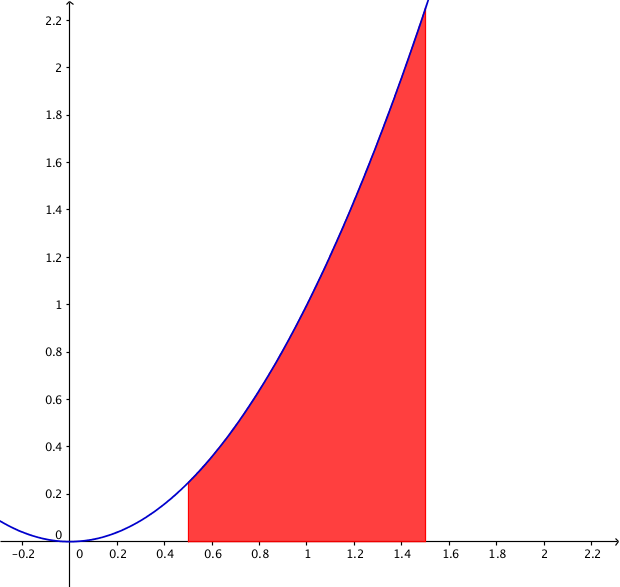
\includegraphics[width=0.8\linewidth, height=0.25\textheight]{integral.png}
        \caption{An example integral of a function.}
\end{figure}
\\In general it is fairly difficult to compute integrals without a smorgasbord of algebraic transformations. However, it is possible to generalize the integral and apply it to mathematical objects other than functions (some of which are actually easier to compute algorithmically)! A \emph{polygonal chain} is a sequence of points $(x_0, y_0), (x_1, y_1), ..., (x_N, y_N)$; every consecutive pair of points gives us a line segment. For example, we draw the the polygonal chain $(1, 5), (3, 7), (5, 2), (10, 9)$ as follows:\\\\
%INSERT PIC HERE
\vspace{-8.37mm}
\begin{figure}[!htb]
    \centering
        \centering
        %\includesvg{integral.svg}
        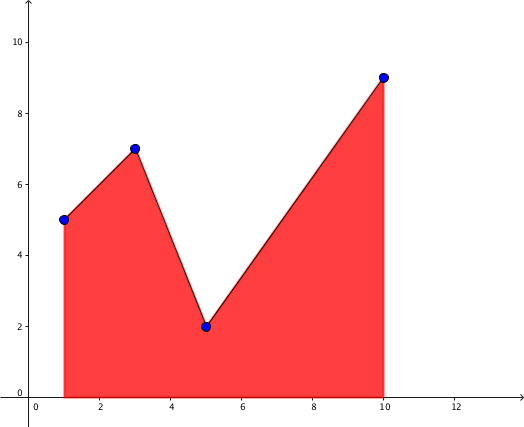
\includegraphics[width=0.8\linewidth, height=0.25\textheight]{polyintegral.png}
        \caption{An example integral of a polygonal chain.}
\end{figure}
\newpage
\noindent
If we restrict ourselves to looking at polygonal chains where $x_0 < x_1 < ... < x_N$, we can then define the integral of this polygonal chain as the area between the $x$-axis and the polygonal chain between $x_0$ and $x_N$.\\\\
Given a polygonal chain, can you compute its integral?
}
\vspace{7mm}\\
\large{\bf{Input}}\vspace{2mm}\\
The input will begin with a line containing a single positive integer, $t$, representing the number of test cases to process. Each test case will begin with an integer $N$ ($2 \leq N \leq 10,000$), the number of points in the polygonal chain. Following will be $N$ lines giving the polygonal chain. The $i$-th line will be of the form ``$x_i \enspace y_i$" ($0 \leq x_i, y_i \leq 10,000$, $x_i$ and $y_i$ are both integers). It is guaranteed that $x_i < x_{i+1}$ for all $i$.
\vspace{3mm}\\
\large{\bf{Output}}\vspace{2mm}\\
For each test case print the area between the given polygonal chain and the $x$-axis rounded to two decimal places on its own line.
\vspace{5mm}\\
\bf{Sample Input} \hspace{52mm} \bf{Sample Output}\vspace{1mm}\\
\begin{tabu*} to 475pt {|X[0r]|X[0l]|}
\tabucline-
\vspace{-\baselineskip} %needs to be placed here
\begin{Verbatim}
1
4
1 5
3 7
5 2
10 9
\end{Verbatim}
&
\vspace{-\baselineskip} %needs to be placed here
\begin{Verbatim}
48.50
\end{Verbatim}
\\
\tabucline-
\end{tabu*}
\end{document}
